\documentclass[12pt]{article}

%packages
%\usepackage{latexsym}
\usepackage{graphicx}
\usepackage{color}
\usepackage{amsmath}
\usepackage{dsfont}
\usepackage{placeins}
\usepackage{amssymb}
\usepackage{wasysym}
\usepackage{abstract}
\usepackage{hyperref}
\usepackage{etoolbox}
\usepackage{datetime}
\usepackage{xcolor}
\usepackage{alphalph}
\settimeformat{ampmtime}

%\usepackage{pstricks,pst-node,pst-tree}

%\usepackage{algpseudocode}
%\usepackage{amsthm}
%\usepackage{hyperref}
%\usepackage{mathrsfs}
%\usepackage{amsfonts}
%\usepackage{bbding}
%\usepackage{listings}
%\usepackage{appendix}
\usepackage[margin=1in]{geometry}
%\geometry{papersize={8.5in,11in},total={6.5in,9in}}
%\usepackage{cancel}
%\usepackage{algorithmic, algorithm}

\makeatletter
\def\maxwidth{ %
  \ifdim\Gin@nat@width>\linewidth
    \linewidth
  \else
    \Gin@nat@width
  \fi
}
\makeatother

\definecolor{fgcolor}{rgb}{0.345, 0.345, 0.345}
\newcommand{\hlnum}[1]{\textcolor[rgb]{0.686,0.059,0.569}{#1}}%
\newcommand{\hlstr}[1]{\textcolor[rgb]{0.192,0.494,0.8}{#1}}%
\newcommand{\hlcom}[1]{\textcolor[rgb]{0.678,0.584,0.686}{\textit{#1}}}%
\newcommand{\hlopt}[1]{\textcolor[rgb]{0,0,0}{#1}}%
\newcommand{\hlstd}[1]{\textcolor[rgb]{0.345,0.345,0.345}{#1}}%
\newcommand{\hlkwa}[1]{\textcolor[rgb]{0.161,0.373,0.58}{\textbf{#1}}}%
\newcommand{\hlkwb}[1]{\textcolor[rgb]{0.69,0.353,0.396}{#1}}%
\newcommand{\hlkwc}[1]{\textcolor[rgb]{0.333,0.667,0.333}{#1}}%
\newcommand{\hlkwd}[1]{\textcolor[rgb]{0.737,0.353,0.396}{\textbf{#1}}}%

\usepackage{framed}
\makeatletter
\newenvironment{kframe}{%
 \def\at@end@of@kframe{}%
 \ifinner\ifhmode%
  \def\at@end@of@kframe{\end{minipage}}%
  \begin{minipage}{\columnwidth}%
 \fi\fi%
 \def\FrameCommand##1{\hskip\@totalleftmargin \hskip-\fboxsep
 \colorbox{shadecolor}{##1}\hskip-\fboxsep
     % There is no \\@totalrightmargin, so:
     \hskip-\linewidth \hskip-\@totalleftmargin \hskip\columnwidth}%
 \MakeFramed {\advance\hsize-\width
   \@totalleftmargin\z@ \linewidth\hsize
   \@setminipage}}%
 {\par\unskip\endMakeFramed%
 \at@end@of@kframe}
\makeatother

\definecolor{shadecolor}{rgb}{.77, .77, .77}
\definecolor{messagecolor}{rgb}{0, 0, 0}
\definecolor{warningcolor}{rgb}{1, 0, 1}
\definecolor{errorcolor}{rgb}{1, 0, 0}
\newenvironment{knitrout}{}{} % an empty environment to be redefined in TeX

\usepackage{alltt}
\usepackage[T1]{fontenc}

\newcommand{\qu}[1]{``#1''}
\newcounter{probnum}
\setcounter{probnum}{1}

%create definition to allow local margin changes
\def\changemargin#1#2{\list{}{\rightmargin#2\leftmargin#1}\item[]}
\let\endchangemargin=\endlist 

%allow equations to span multiple pages
\allowdisplaybreaks

%define colors and color typesetting conveniences
\definecolor{gray}{rgb}{0.5,0.5,0.5}
\definecolor{black}{rgb}{0,0,0}
\definecolor{white}{rgb}{1,1,1}
\definecolor{blue}{rgb}{0.5,0.5,1}
\newcommand{\inblue}[1]{\color{blue}#1 \color{black}}
\definecolor{green}{rgb}{0.133,0.545,0.133}
\newcommand{\ingreen}[1]{\color{green}#1 \color{black}}
\definecolor{yellow}{rgb}{1,1,0}
\newcommand{\inyellow}[1]{\color{yellow}#1 \color{black}}
\definecolor{orange}{rgb}{0.9,0.649,0}
\newcommand{\inorange}[1]{\color{orange}#1 \color{black}}
\definecolor{red}{rgb}{1,0.133,0.133}
\newcommand{\inred}[1]{\color{red}#1 \color{black}}
\definecolor{purple}{rgb}{0.58,0,0.827}
\newcommand{\inpurple}[1]{\color{purple}#1 \color{black}}
\definecolor{backgcode}{rgb}{0.97,0.97,0.8}
\definecolor{Brown}{cmyk}{0,0.81,1,0.60}
\definecolor{OliveGreen}{cmyk}{0.64,0,0.95,0.40}
\definecolor{CadetBlue}{cmyk}{0.62,0.57,0.23,0}

%define new math operators
\DeclareMathOperator*{\argmax}{arg\,max~}
\DeclareMathOperator*{\argmin}{arg\,min~}
\DeclareMathOperator*{\argsup}{arg\,sup~}
\DeclareMathOperator*{\arginf}{arg\,inf~}
\DeclareMathOperator*{\convolution}{\text{\Huge{$\ast$}}}
\newcommand{\infconv}[2]{\convolution^\infty_{#1 = 1} #2}
%true functions

%%%% GENERAL SHORTCUTS

%shortcuts for pure typesetting conveniences
\newcommand{\bv}[1]{\boldsymbol{#1}}

%shortcuts for compound constants
\newcommand{\BetaDistrConst}{\dfrac{\Gamma(\alpha + \beta)}{\Gamma(\alpha)\Gamma(\beta)}}
\newcommand{\NormDistrConst}{\dfrac{1}{\sqrt{2\pi\sigma^2}}}

%shortcuts for conventional symbols
\newcommand{\tsq}{\tau^2}
\newcommand{\tsqh}{\hat{\tau}^2}
\newcommand{\sigsq}{\sigma^2}
\newcommand{\sigsqsq}{\parens{\sigma^2}^2}
\newcommand{\sigsqovern}{\dfrac{\sigsq}{n}}
\newcommand{\tausq}{\tau^2}
\newcommand{\tausqalpha}{\tau^2_\alpha}
\newcommand{\tausqbeta}{\tau^2_\beta}
\newcommand{\tausqsigma}{\tau^2_\sigma}
\newcommand{\betasq}{\beta^2}
\newcommand{\sigsqvec}{\bv{\sigma}^2}
\newcommand{\sigsqhat}{\hat{\sigma}^2}
\newcommand{\sigsqhatmlebayes}{\sigsqhat_{\text{Bayes, MLE}}}
\newcommand{\sigsqhatmle}[1]{\sigsqhat_{#1, \text{MLE}}}
\newcommand{\bSigma}{\bv{\Sigma}}
\newcommand{\bSigmainv}{\bSigma^{-1}}
\newcommand{\thetavec}{\bv{\theta}}
\newcommand{\thetahat}{\hat{\theta}}
\newcommand{\thetahatmle}{\hat{\theta}_{\mathrm{MLE}}}
\newcommand{\thetavechatmle}{\hat{\thetavec}_{\mathrm{MLE}}}
\newcommand{\muhat}{\hat{\mu}}
\newcommand{\musq}{\mu^2}
\newcommand{\muvec}{\bv{\mu}}
\newcommand{\muhatmle}{\muhat_{\text{MLE}}}
\newcommand{\lambdahat}{\hat{\lambda}}
\newcommand{\lambdahatmle}{\lambdahat_{\text{MLE}}}
\newcommand{\etavec}{\bv{\eta}}
\newcommand{\alphavec}{\bv{\alpha}}
\newcommand{\minimaxdec}{\delta^*_{\mathrm{mm}}}
\newcommand{\ybar}{\bar{y}}
\newcommand{\xbar}{\bar{x}}
\newcommand{\Xbar}{\bar{X}}
\newcommand{\phat}{\hat{p}}
\newcommand{\Phat}{\hat{P}}
\newcommand{\Zbar}{\bar{Z}}
\newcommand{\iid}{~{\buildrel iid \over \sim}~}
\newcommand{\inddist}{~{\buildrel ind \over \sim}~}
\newcommand{\approxdist}{~{\buildrel approx \over \sim}~}
\newcommand{\equalsindist}{~{\buildrel d \over =}~}
\newcommand{\loglik}[1]{\ell\parens{#1}}
\newcommand{\thetahatkminone}{\thetahat^{(k-1)}}
\newcommand{\thetahatkplusone}{\thetahat^{(k+1)}}
\newcommand{\thetahatk}{\thetahat^{(k)}}
\newcommand{\half}{\frac{1}{2}}
\newcommand{\third}{\frac{1}{3}}
\newcommand{\twothirds}{\frac{2}{3}}
\newcommand{\fourth}{\frac{1}{4}}
\newcommand{\fifth}{\frac{1}{5}}
\newcommand{\sixth}{\frac{1}{6}}

%shortcuts for vector and matrix notation
\newcommand{\A}{\bv{A}}
\newcommand{\At}{\A^T}
\newcommand{\Ainv}{\inverse{\A}}
\newcommand{\B}{\bv{B}}
\newcommand{\K}{\bv{K}}
\newcommand{\Kt}{\K^T}
\newcommand{\Kinv}{\inverse{K}}
\newcommand{\Kinvt}{(\Kinv)^T}
\newcommand{\M}{\bv{M}}
\newcommand{\Bt}{\B^T}
\newcommand{\Q}{\bv{Q}}
\newcommand{\Qt}{\Q^T}
\newcommand{\R}{\bv{R}}
\newcommand{\Rt}{\R^T}
\newcommand{\Z}{\bv{Z}}
\newcommand{\X}{\bv{X}}
\newcommand{\Xsub}{\X_{\text{(sub)}}}
\newcommand{\Xsubadj}{\X_{\text{(sub,adj)}}}
\newcommand{\I}{\bv{I}}
\newcommand{\Y}{\bv{Y}}
\newcommand{\sigsqI}{\sigsq\I}
\renewcommand{\P}{\bv{P}}
\newcommand{\Psub}{\P_{\text{(sub)}}}
\newcommand{\Pt}{\P^T}
\newcommand{\Pii}{P_{ii}}
\newcommand{\Pij}{P_{ij}}
\newcommand{\IminP}{(\I-\P)}
\newcommand{\Xt}{\bv{X}^T}
\newcommand{\XtX}{\Xt\X}
\newcommand{\XtXinv}{\parens{\Xt\X}^{-1}}
\newcommand{\XtXinvXt}{\XtXinv\Xt}
\newcommand{\XXtXinvXt}{\X\XtXinvXt}
\newcommand{\x}{\bv{x}}
\renewcommand{\b}{\bv{b}}
\newcommand{\onevec}{\bv{1}}
\newcommand{\oneton}{1, \ldots, n}
\newcommand{\yoneton}{y_1, \ldots, y_n}
\newcommand{\yonetonorder}{y_{(1)}, \ldots, y_{(n)}}
\newcommand{\Yoneton}{Y_1, \ldots, Y_n}
\newcommand{\iinoneton}{i \in \braces{\oneton}}
\newcommand{\onetom}{1, \ldots, m}
\newcommand{\jinonetom}{j \in \braces{\onetom}}
\newcommand{\xoneton}{x_1, \ldots, x_n}
\newcommand{\Xoneton}{X_1, \ldots, X_n}
\newcommand{\xt}{\x^T}
\newcommand{\y}{\bv{y}}
\newcommand{\yt}{\y^T}
\renewcommand{\c}{\bv{c}}
\newcommand{\ct}{\c^T}
\newcommand{\tstar}{\bv{t}^*}
\renewcommand{\u}{\bv{u}}
\renewcommand{\v}{\bv{v}}
\renewcommand{\a}{\bv{a}}
\newcommand{\s}{\bv{s}}
\newcommand{\yadj}{\y_{\text{(adj)}}}
\newcommand{\xjadj}{\x_{j\text{(adj)}}}
\newcommand{\xjadjM}{\x_{j \perp M}}
\newcommand{\yhat}{\hat{\y}}
\newcommand{\yhatsub}{\yhat_{\text{(sub)}}}
\newcommand{\yhatstar}{\yhat^*}
\newcommand{\yhatstarnew}{\yhatstar_{\text{new}}}
\newcommand{\z}{\bv{z}}
\newcommand{\zt}{\z^T}
\newcommand{\bb}{\bv{b}}
\newcommand{\bbt}{\bb^T}
\newcommand{\bbeta}{\bv{\beta}}
\newcommand{\beps}{\bv{\epsilon}}
\newcommand{\bepst}{\beps^T}
\newcommand{\e}{\bv{e}}
\newcommand{\Mofy}{\M(\y)}
\newcommand{\KofAlpha}{K(\alpha)}
\newcommand{\ellset}{\mathcal{L}}
\newcommand{\oneminalph}{1-\alpha}
\newcommand{\SSE}{\text{SSE}}
\newcommand{\SSEsub}{\text{SSE}_{\text{(sub)}}}
\newcommand{\MSE}{\text{MSE}}
\newcommand{\RMSE}{\text{RMSE}}
\newcommand{\SSR}{\text{SSR}}
\newcommand{\SST}{\text{SST}}
\newcommand{\JSest}{\delta_{\text{JS}}(\x)}
\newcommand{\Bayesest}{\delta_{\text{Bayes}}(\x)}
\newcommand{\EmpBayesest}{\delta_{\text{EmpBayes}}(\x)}
\newcommand{\BLUPest}{\delta_{\text{BLUP}}}
\newcommand{\MLEest}[1]{\hat{#1}_{\text{MLE}}}

%shortcuts for Linear Algebra stuff (i.e. vectors and matrices)
\newcommand{\twovec}[2]{\bracks{\begin{array}{c} #1 \\ #2 \end{array}}}
\newcommand{\threevec}[3]{\bracks{\begin{array}{c} #1 \\ #2 \\ #3 \end{array}}}
\newcommand{\fivevec}[5]{\bracks{\begin{array}{c} #1 \\ #2 \\ #3 \\ #4 \\ #5 \end{array}}}
\newcommand{\twobytwomat}[4]{\bracks{\begin{array}{cc} #1 & #2 \\ #3 & #4 \end{array}}}
\newcommand{\threebytwomat}[6]{\bracks{\begin{array}{cc} #1 & #2 \\ #3 & #4 \\ #5 & #6 \end{array}}}

%shortcuts for conventional compound symbols
\newcommand{\thetainthetas}{\theta \in \Theta}
\newcommand{\reals}{\mathbb{R}}
\newcommand{\complexes}{\mathbb{C}}
\newcommand{\rationals}{\mathbb{Q}}
\newcommand{\integers}{\mathbb{Z}}
\newcommand{\naturals}{\mathbb{N}}
\newcommand{\forallninN}{~~\forall n \in \naturals}
\newcommand{\forallxinN}[1]{~~\forall #1 \in \reals}
\newcommand{\matrixdims}[2]{\in \reals^{\,#1 \times #2}}
\newcommand{\inRn}[1]{\in \reals^{\,#1}}
\newcommand{\mathimplies}{\quad\Rightarrow\quad}
\newcommand{\mathlogicequiv}{\quad\Leftrightarrow\quad}
\newcommand{\eqncomment}[1]{\quad \text{(#1)}}
\newcommand{\limitn}{\lim_{n \rightarrow \infty}}
\newcommand{\limitN}{\lim_{N \rightarrow \infty}}
\newcommand{\limitd}{\lim_{d \rightarrow \infty}}
\newcommand{\limitt}{\lim_{t \rightarrow \infty}}
\newcommand{\limitsupn}{\limsup_{n \rightarrow \infty}~}
\newcommand{\limitinfn}{\liminf_{n \rightarrow \infty}~}
\newcommand{\limitk}{\lim_{k \rightarrow \infty}}
\newcommand{\limsupn}{\limsup_{n \rightarrow \infty}}
\newcommand{\limsupk}{\limsup_{k \rightarrow \infty}}
\newcommand{\floor}[1]{\left\lfloor #1 \right\rfloor}
\newcommand{\ceil}[1]{\left\lceil #1 \right\rceil}

%shortcuts for environments
\newcommand{\beqn}{\vspace{-0.25cm}\begin{eqnarray*}}
\newcommand{\eeqn}{\end{eqnarray*}}
\newcommand{\bneqn}{\vspace{-0.25cm}\begin{eqnarray}}
\newcommand{\eneqn}{\end{eqnarray}}

%shortcuts for mini environments
\newcommand{\parens}[1]{\left(#1\right)}
\newcommand{\squared}[1]{\parens{#1}^2}
\newcommand{\tothepow}[2]{\parens{#1}^{#2}}
\newcommand{\prob}[1]{\mathbb{P}\parens{#1}}
\newcommand{\cprob}[2]{\prob{#1~|~#2}}
\newcommand{\littleo}[1]{o\parens{#1}}
\newcommand{\bigo}[1]{O\parens{#1}}
\newcommand{\Lp}[1]{\mathbb{L}^{#1}}
\renewcommand{\arcsin}[1]{\text{arcsin}\parens{#1}}
\newcommand{\prodonen}[2]{\bracks{\prod_{#1=1}^n #2}}
\newcommand{\mysum}[4]{\sum_{#1=#2}^{#3} #4}
\newcommand{\sumonen}[2]{\sum_{#1=1}^n #2}
\newcommand{\infsum}[2]{\sum_{#1=1}^\infty #2}
\newcommand{\infprod}[2]{\prod_{#1=1}^\infty #2}
\newcommand{\infunion}[2]{\bigcup_{#1=1}^\infty #2}
\newcommand{\infinter}[2]{\bigcap_{#1=1}^\infty #2}
\newcommand{\infintegral}[2]{\int^\infty_{-\infty} #2 ~\text{d}#1}
\newcommand{\supthetas}[1]{\sup_{\thetainthetas}\braces{#1}}
\newcommand{\bracks}[1]{\left[#1\right]}
\newcommand{\braces}[1]{\left\{#1\right\}}
\newcommand{\set}[1]{\left\{#1\right\}}
\newcommand{\abss}[1]{\left|#1\right|}
\newcommand{\norm}[1]{\left|\left|#1\right|\right|}
\newcommand{\normsq}[1]{\norm{#1}^2}
\newcommand{\inverse}[1]{\parens{#1}^{-1}}
\newcommand{\rowof}[2]{\parens{#1}_{#2\cdot}}

%shortcuts for functionals
\newcommand{\realcomp}[1]{\text{Re}\bracks{#1}}
\newcommand{\imagcomp}[1]{\text{Im}\bracks{#1}}
\newcommand{\range}[1]{\text{range}\bracks{#1}}
\newcommand{\colsp}[1]{\text{colsp}\bracks{#1}}
\newcommand{\rowsp}[1]{\text{rowsp}\bracks{#1}}
\newcommand{\tr}[1]{\text{tr}\bracks{#1}}
\newcommand{\rank}[1]{\text{rank}\bracks{#1}}
\newcommand{\proj}[2]{\text{Proj}_{#1}\bracks{#2}}
\newcommand{\projcolspX}[1]{\text{Proj}_{\colsp{\X}}\bracks{#1}}
\newcommand{\median}[1]{\text{median}\bracks{#1}}
\newcommand{\mean}[1]{\text{mean}\bracks{#1}}
\newcommand{\dime}[1]{\text{dim}\bracks{#1}}
\renewcommand{\det}[1]{\text{det}\bracks{#1}}
\newcommand{\expe}[1]{\mathbb{E}\bracks{#1}}
\newcommand{\expeabs}[1]{\expe{\abss{#1}}}
\newcommand{\expesub}[2]{\mathbb{E}_{#1}\bracks{#2}}
\newcommand{\indic}[1]{\mathds{1}_{#1}}
\newcommand{\var}[1]{\mathbb{V}\text{ar}\bracks{#1}}
\newcommand{\cov}[2]{\mathbb{C}\text{ov}\bracks{#1, #2}}
\newcommand{\corr}[2]{\text{Corr}\bracks{#1, #2}}
\newcommand{\se}[1]{\mathbb{S}\text{E}\bracks{#1}}
\newcommand{\seest}[1]{\hat{\mathbb{S}\text{E}}\bracks{#1}}
\newcommand{\bias}[1]{\text{Bias}\bracks{#1}}
\newcommand{\derivop}[2]{\dfrac{\text{d}}{\text{d} #1}\bracks{#2}}
\newcommand{\partialop}[2]{\dfrac{\partial}{\partial #1}\bracks{#2}}
\newcommand{\secpartialop}[2]{\dfrac{\partial^2}{\partial #1^2}\bracks{#2}}
\newcommand{\mixpartialop}[3]{\dfrac{\partial^2}{\partial #1 \partial #2}\bracks{#3}}

%shortcuts for functions
\renewcommand{\exp}[1]{\mathrm{exp}\parens{#1}}
\renewcommand{\cos}[1]{\text{cos}\parens{#1}}
\renewcommand{\sin}[1]{\text{sin}\parens{#1}}
\newcommand{\sign}[1]{\text{sign}\parens{#1}}
\newcommand{\are}[1]{\mathrm{ARE}\parens{#1}}
\newcommand{\natlog}[1]{\ln\parens{#1}}
\newcommand{\oneover}[1]{\frac{1}{#1}}
\newcommand{\overtwo}[1]{\frac{#1}{2}}
\newcommand{\overn}[1]{\frac{#1}{n}}
\newcommand{\oneoversqrt}[1]{\oneover{\sqrt{#1}}}
\newcommand{\sqd}[1]{\parens{#1}^2}
\newcommand{\loss}[1]{\ell\parens{\theta, #1}}
\newcommand{\losstwo}[2]{\ell\parens{#1, #2}}
\newcommand{\cf}{\phi(t)}

%English language specific shortcuts
\newcommand{\ie}{\textit{i.e.} }
\newcommand{\AKA}{\textit{AKA} }
\renewcommand{\iff}{\textit{iff}}
\newcommand{\eg}{\textit{e.g.} }
\newcommand{\st}{\textit{s.t.} }
\newcommand{\wrt}{\textit{w.r.t.} }
\newcommand{\mathst}{~~\text{\st}~~}
\newcommand{\mathand}{~~\text{and}~~}
\newcommand{\ala}{\textit{a la} }
\newcommand{\ppp}{posterior predictive p-value}
\newcommand{\dd}{dataset-to-dataset}

%shortcuts for distribution titles
\newcommand{\logistic}[2]{\mathrm{Logistic}\parens{#1,\,#2}}
\newcommand{\bernoulli}[1]{\mathrm{Bernoulli}\parens{#1}}
\newcommand{\betanot}[2]{\mathrm{Beta}\parens{#1,\,#2}}
\newcommand{\stdbetanot}{\betanot{\alpha}{\beta}}
\newcommand{\multnormnot}[3]{\mathcal{N}_{#1}\parens{#2,\,#3}}
\newcommand{\normnot}[2]{\mathcal{N}\parens{#1,\,#2}}
\newcommand{\classicnormnot}{\normnot{\mu}{\sigsq}}
\newcommand{\stdnormnot}{\normnot{0}{1}}
\newcommand{\uniformdiscrete}[1]{\mathrm{Uniform}\parens{\braces{#1}}}
\newcommand{\uniform}[2]{\mathrm{U}\parens{#1,\,#2}}
\newcommand{\stduniform}{\uniform{0}{1}}
\newcommand{\geometric}[1]{\mathrm{Geometric}\parens{#1}}
\newcommand{\hypergeometric}[3]{\mathrm{Hypergeometric}\parens{#1,\,#2,\,#3}}
\newcommand{\exponential}[1]{\mathrm{Exp}\parens{#1}}
\newcommand{\gammadist}[2]{\mathrm{Gamma}\parens{#1, #2}}
\newcommand{\poisson}[1]{\mathrm{Poisson}\parens{#1}}
\newcommand{\binomial}[2]{\mathrm{Binomial}\parens{#1,\,#2}}
\newcommand{\negbin}[2]{\mathrm{NegBin}\parens{#1,\,#2}}
\newcommand{\rayleigh}[1]{\mathrm{Rayleigh}\parens{#1}}
\newcommand{\multinomial}[2]{\mathrm{Multinomial}\parens{#1,\,#2}}
\newcommand{\gammanot}[2]{\mathrm{Gamma}\parens{#1,\,#2}}
\newcommand{\cauchynot}[2]{\text{Cauchy}\parens{#1,\,#2}}
\newcommand{\invchisqnot}[1]{\text{Inv}\chisq{#1}}
\newcommand{\invscaledchisqnot}[2]{\text{ScaledInv}\ncchisq{#1}{#2}}
\newcommand{\invgammanot}[2]{\text{InvGamma}\parens{#1,\,#2}}
\newcommand{\chisq}[1]{\chi^2_{#1}}
\newcommand{\ncchisq}[2]{\chi^2_{#1}\parens{#2}}
\newcommand{\ncF}[3]{F_{#1,#2}\parens{#3}}

%shortcuts for PDF's of common distributions
\newcommand{\logisticpdf}[3]{\oneover{#3}\dfrac{\exp{-\dfrac{#1 - #2}{#3}}}{\parens{1+\exp{-\dfrac{#1 - #2}{#3}}}^2}}
\newcommand{\betapdf}[3]{\dfrac{\Gamma(#2 + #3)}{\Gamma(#2)\Gamma(#3)}#1^{#2-1} (1-#1)^{#3-1}}
\newcommand{\normpdf}[3]{\frac{1}{\sqrt{2\pi#3}}\exp{-\frac{1}{2#3}(#1 - #2)^2}}
\newcommand{\normpdfvarone}[2]{\dfrac{1}{\sqrt{2\pi}}e^{-\half(#1 - #2)^2}}
\newcommand{\chisqpdf}[2]{\dfrac{1}{2^{#2/2}\Gamma(#2/2)}\; {#1}^{#2/2-1} e^{-#1/2}}
\newcommand{\invchisqpdf}[2]{\dfrac{2^{-\overtwo{#1}}}{\Gamma(#2/2)}\,{#1}^{-\overtwo{#2}-1}  e^{-\oneover{2 #1}}}
\newcommand{\exponentialpdf}[2]{#2\exp{-#2#1}}
\newcommand{\poissonpdf}[2]{\dfrac{e^{-#1} #1^{#2}}{#2!}}
\newcommand{\binomialpdf}[3]{\binom{#2}{#1}#3^{#1}(1-#3)^{#2-#1}}
\newcommand{\rayleighpdf}[2]{\dfrac{#1}{#2^2}\exp{-\dfrac{#1^2}{2 #2^2}}}
\newcommand{\gammapdf}[3]{\dfrac{#3^#2}{\Gamma\parens{#2}}#1^{#2-1}\exp{-#3 #1}}
\newcommand{\cauchypdf}[3]{\oneover{\pi} \dfrac{#3}{\parens{#1-#2}^2 + #3^2}}
\newcommand{\Gammaf}[1]{\Gamma\parens{#1}}

%shortcuts for miscellaneous typesetting conveniences
\newcommand{\notesref}[1]{\marginpar{\color{gray}\tt #1\color{black}}}

%%%% DOMAIN-SPECIFIC SHORTCUTS

%Real analysis related shortcuts
\newcommand{\zeroonecl}{\bracks{0,1}}
\newcommand{\forallepsgrzero}{\forall \epsilon > 0~~}
\newcommand{\lessthaneps}{< \epsilon}
\newcommand{\fraccomp}[1]{\text{frac}\bracks{#1}}

%Bayesian related shortcuts
\newcommand{\yrep}{y^{\text{rep}}}
\newcommand{\yrepisq}{(\yrep_i)^2}
\newcommand{\yrepvec}{\bv{y}^{\text{rep}}}


%Probability shortcuts
\newcommand{\SigField}{\mathcal{F}}
\newcommand{\ProbMap}{\mathcal{P}}
\newcommand{\probtrinity}{\parens{\Omega, \SigField, \ProbMap}}
\newcommand{\convp}{~{\buildrel p \over \rightarrow}~}
\newcommand{\convLp}[1]{~{\buildrel \Lp{#1} \over \rightarrow}~}
\newcommand{\nconvp}{~{\buildrel p \over \nrightarrow}~}
\newcommand{\convae}{~{\buildrel a.e. \over \longrightarrow}~}
\newcommand{\convau}{~{\buildrel a.u. \over \longrightarrow}~}
\newcommand{\nconvau}{~{\buildrel a.u. \over \nrightarrow}~}
\newcommand{\nconvae}{~{\buildrel a.e. \over \nrightarrow}~}
\newcommand{\convd}{~{\buildrel \mathcal{D} \over \rightarrow}~}
\newcommand{\nconvd}{~{\buildrel \mathcal{D} \over \nrightarrow}~}
\newcommand{\withprob}{~~\text{w.p.}~~}
\newcommand{\io}{~~\text{i.o.}}

\newcommand{\Acl}{\bar{A}}
\newcommand{\ENcl}{\bar{E}_N}
\newcommand{\diam}[1]{\text{diam}\parens{#1}}

\newcommand{\taua}{\tau_a}

\newcommand{\myint}[4]{\int_{#2}^{#3} #4 \,\text{d}#1}
\newcommand{\laplacet}[1]{\mathscr{L}\bracks{#1}}
\newcommand{\laplaceinvt}[1]{\mathscr{L}^{-1}\bracks{#1}}
\renewcommand{\min}[1]{\text{min}\braces{#1}}
\renewcommand{\max}[1]{\text{max}\braces{#1}}

\newcommand{\Vbar}[1]{\bar{V}\parens{#1}}
\newcommand{\expnegrtau}{\exp{-r\tau}}

%%% problem typesetting
\definecolor{darkgrey}{rgb}{0.10,0.10,0.9}

\newcommand{\problem}[1]{\noindent \colorbox{black}{{\color{yellow} \large{\textsf{\textbf{Problem \arabic{probnum}}}}~}} \addtocounter{probnum}{1} \vspace{0.2cm} \\ \iftoggle{professormode}{}{\color{darkgrey}} #1}

\newcommand{\easysubproblem}[1]{\ingreen{\item} \iftoggle{professormode}{}{\color{darkgrey}} [easy] #1 \color{black} }
\newcommand{\intermediatesubproblem}[1]{\inorange{\item} \iftoggle{professormode}{}{\color{darkgrey}} [harder] #1 \color{black} }
\newcommand{\hardsubproblem}[1]{\inred{\item} \iftoggle{professormode}{}{\color{darkgrey}} [difficult] #1 \color{black} }
\newcommand{\extracreditsubproblem}[1]{\inpurple{\item} \iftoggle{professormode}{}{\color{darkgrey}} [E.C.] #1 \color{black} }


\newcommand{\spc}[1]{\iftoggle{professormode}{\\ \vspace{#1cm}}{\\ \vspace{-0.3cm}}}

\makeatletter
\newalphalph{\alphmult}[mult]{\@alph}{26}
\renewcommand{\labelenumi}{(\alphmult{\value{enumi}})}

\newcommand{\support}[1]{\text{Supp}\bracks{#1}}
\newcommand{\mode}[1]{\text{Mode}\bracks{#1}}
\newcommand{\IQR}[1]{\text{IQR}\bracks{#1}}
\newcommand{\quantile}[2]{\text{Quantile}\bracks{#1,\,#2}}


\newtoggle{professormode}



\title{MATH 342W / 642 / RM 742 Spring \the\year~ HW \#5}

\author{Mohammed Z Hasan} %STUDENTS: write your name here

\iftoggle{professormode}{
\date{Due 11:59PM May 15 \\ \vspace{0.5cm} \small (this document last updated \currenttime~on \today)}
}

\renewcommand{\abstractname}{Instructions and Philosophy}

\begin{document}
\maketitle

\iftoggle{professormode}{
\begin{abstract}
The path to success in this class is to do many problems. Unlike other courses, exclusively doing reading(s) will not help. Coming to lecture is akin to watching workout videos; thinking about and solving problems on your own is the actual ``working out.''  Feel free to \qu{work out} with others; \textbf{I want you to work on this in groups.}

Reading is still \textit{required}. You should be googling and reading about all the concepts introduced in class online. This is your responsibility to supplement in-class with your own readings.

The problems below are color coded: \ingreen{green} problems are considered \textit{easy} and marked \qu{[easy]}; \inorange{yellow} problems are considered \textit{intermediate} and marked \qu{[harder]}, \inred{red} problems are considered \textit{difficult} and marked \qu{[difficult]} and \inpurple{purple} problems are extra credit. The \textit{easy} problems are intended to be ``giveaways'' if you went to class. Do as much as you can of the others; I expect you to at least attempt the \textit{difficult} problems. 

This homework is worth 100 points but the point distribution will not be determined until after the due date. See syllabus for the policy on late homework.

Up to 7 points are given as a bonus if the homework is typed using \LaTeX. Links to instaling \LaTeX~and program for compiling \LaTeX~is found on the syllabus. You are encouraged to use \url{overleaf.com}. If you are handing in homework this way, read the comments in the code; there are two lines to comment out and you should replace my name with yours and write your section. The easiest way to use overleaf is to copy the raw text from hwxx.tex and preamble.tex into two new overleaf tex files with the same name. If you are asked to make drawings, you can take a picture of your handwritten drawing and insert them as figures or leave space using the \qu{$\backslash$vspace} command and draw them in after printing or attach them stapled.

The document is available with spaces for you to write your answers. If not using \LaTeX, print this document and write in your answers. I do not accept homeworks which are \textit{not} on this printout. Keep this first page printed for your records.

\end{abstract}

\thispagestyle{empty}
\vspace{1cm}
NAME: \line(1,0){380}
\clearpage
}




\problem{These are some questions related to probability estimation modeling and asymmetric cost modeling.}

\begin{enumerate}
\easysubproblem{Why is logistic regression an example of a \qu{generalized linear model} (glm)?}\spc{3}

Logistic regression is considered a type of generalized linear model (GLM) because it extends the linear regression framework to model binary response variables by using a link function. In logistic regression, the response variable \( Y \) is binary, and the model predicts the probability that \( Y = 1 \) given a set of predictors \( X \).


\easysubproblem{What is $\mathcal{H}_{pr}$ for the probability estimation algorithm that employs the linear model in the covariates with logistic link function?}\spc{2}

\[
H_{\text{pr}} = \left\{ p(x) = \frac{1}{1 + e^{-\beta^T x}} : \beta \in \mathbb{R}^d \right\}
\]

where \(\beta\) represents the vector of coefficients, \(x\) the vector of covariates, and \(d\) the number of covariates.


\easysubproblem{If logistic regression predicts 3.1415 for a new $\x_*$, what is the probability estimate that $y=1$ for this $\x_*$?}\spc{2}

To find the probability estimate \(p(y=1 \mid x^*)\), we apply the logistic function:
\[
p(y=1 \mid x^*) = \frac{1}{1 + e^{-\beta^T x^*}} = \frac{1}{1 + e^{-3.1415}}
\]

Let's calculate the specific probability:
\[
p(y=1 \mid x^*) = \frac{1}{1 + e^{-3.1415}}
\]


\intermediatesubproblem{What is $\mathcal{H}_{pr}$ for the probability estimation algorithm that employs the linear model in the covariates with cloglog link function?}\spc{5}

The \textit{cloglog} is used typically for modeling count data where events happen independently with a constant known rate. It’s another example of a generalized linear model (GLM). The cloglog function is defined as:
\[
\log(-\log(1-p)) = \beta^T x
\]
where \(p\) is the probability of \(Y=1\) given \(x\), and \(\beta\) is the vector of coefficients.

The hypothesis space \(H_{\text{pr}}\) for this model includes all functions of the form:
\[
H_{\text{pr}} = \{p(x) = 1 - \exp(-\exp(\beta^T x)) : \beta \in \mathbb{R}^d\}
\]


\hardsubproblem{Generalize linear probability estimation to the case where $\mathcal{Y} = \braces{C_1, C_2, C_3}$. Use the logistic link function like in logistic regression. Write down the objective function that you would numerically maximize. This objective function is one that is argmax'd over the parameters (you define what these parameters are --- that is part of the question). 

Once you get the answer you can see how this easily goes to $K > 3$ response categories. The algorithm for general $K$ is known as \qu{multinomial logistic regression}, \qu{polytomous LR}, \qu{multiclass LR}, \qu{softmax regression}, \qu{multinomial logit} (mlogit), the \qu{maximum entropy} (MaxEnt) classifier, and the \qu{conditional maximum entropy model}. You can inflate your resume with lots of jazz by doing this one question!}\spc{12}

Let \(\mathbf{X}\) be the feature vector for an observation. The probability of an observation belonging to class \(C_k\) is modeled as:

\[
P(Y = C_k \mid \mathbf{X}) = \frac{\exp(\boldsymbol{\beta}_k^\top \mathbf{X})}{\sum_{j=1}^{3} \exp(\boldsymbol{\beta}_j^\top \mathbf{X})}
\]

Objective Function:

The objective is to maximize the log-likelihood of the observed data. Let \(\{(\mathbf{X}_i, Y_i)\}_{i=1}^{n}\) be the dataset, where \(Y_i \in \{C_1, C_2, C_3\}\). The log-likelihood function \(L\) is:

\[
L(\boldsymbol{\beta}) = \sum_{i=1}^{n} \sum_{k=1}^{3} I(Y_i = C_k) \log P(Y_i = C_k \mid \mathbf{X}_i)
\]
For \(K\) classes, the objective function remains similar:

\[
L(\boldsymbol{\beta}) = \sum_{i=1}^{n} \sum_{k=1}^{K} I(Y_i = C_k) \left[ \boldsymbol{\beta}_k^\top \mathbf{X}_i - \log \left( \sum_{j=1}^{K} \exp(\boldsymbol{\beta}_j^\top \mathbf{X}_i) \right) \right]
\]

\easysubproblem{Graph a canonical ROC and label the axes. In your drawing estimate AUC. Explain very clearly what is measured by the $x$ axis and the $y$ axis.}\spc{7}

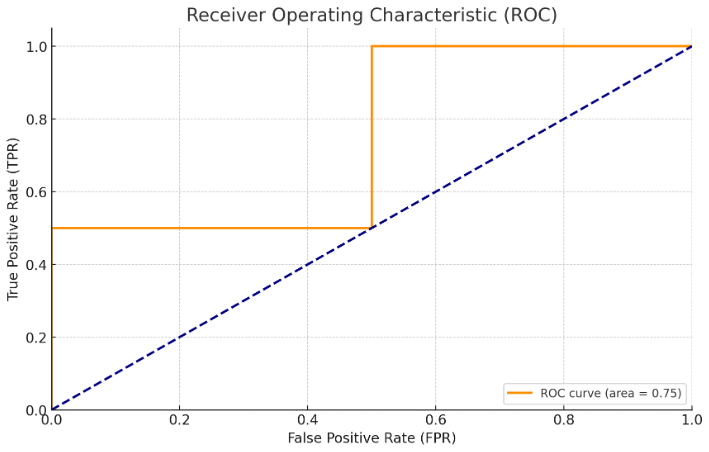
\includegraphics[scale=0.8]{hw05graph.png}

X-axis (False Positive Rate - FPR):

This measures the proportion of negative samples that are incorrectly classified as positive. It is calculated as:

\[
\text{FPR} = \frac{\text{False Positives}}{\text{False Positives} + \text{True Negatives}}
\]

A lower FPR indicates fewer negative samples are misclassified as positive.

Y-axis (True Positive Rate - TPR):

This measures the proportion of positive samples that are correctly classified as positive. It is also known as sensitivity or recall. It is calculated as:

\[
\text{TPR} = \frac{\text{True Positives}}{\text{True Positives} + \text{False Negatives}}
\]

\easysubproblem{Pick one point on your ROC curve from the previous question. Explain a situation why you would employ this model.}\spc{3}

Im choosing: TPR = 0.5 and FPR = 0.2. Employing this model in a medical screening context is justified because it achieves a balance between correctly identifying a substantial number of true positives and keeping the false positive rate at a manageable level.

\intermediatesubproblem{Graph a canonical DET curve and label the axes. Explain very clearly what is measured by the $x$ axis and the $y$ axis. Make sure the DET curve's intersections with the axes is correct.}\spc{7}


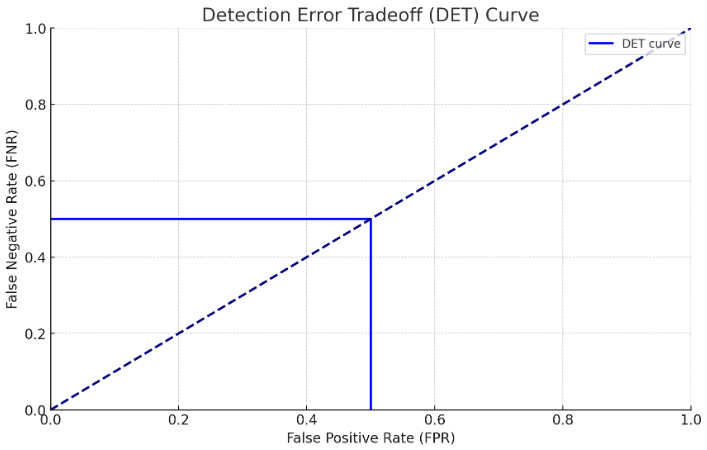
\includegraphics[scale=0.8]{hw05graph2.png}

X-axis (False Positive Rate - FPR):

This measures the proportion of negative samples that are incorrectly classified as positive. It is calculated as:

\[
\text{FPR} = \frac{\text{False Positives}}{\text{False Positives} + \text{True Negatives}}
\]

A lower FPR indicates fewer negative samples are misclassified as positive.

Y-axis (False Negative Rate - FNR):

This measures the proportion of positive samples that are incorrectly classified as negative. It is calculated as:

\[
\text{FNR} = \frac{\text{False Negatives}}{\text{False Negatives} + \text{True Positives}}
\]

\easysubproblem{Pick one point on your DET curve from the previous question. Explain a situation why you would employ this model.}\spc{3}

I chose FPR = 0.3 and FNR = 0.2. Using this model for security screening at an airport makes sense because it strikes a good balance: it catches most potential threats (low FNR) while keeping the number of unnecessary additional screenings (moderate FPR) manageable.

\hardsubproblem{[MA] The line of random guessing on the ROC curve is the diagonal line with slope one extending from the origin. What is the corresponding line of random guessing in the DET curve? This is not easy...}\spc{5}
\end{enumerate}



\problem{These are some questions related to bias-variance decomposition. Assume the two assumptions from the notes about the random variable model that produces the $\delta$ values, the error due to ignorance.}

\begin{enumerate}
\easysubproblem{Write down (do not derive) the decomposition of MSE for a given $\x_*$ where $\mathbb{D}$ is assumed fixed but the response associated with $\x_*$ is assumed random.}\spc{1}

When the dataset \(D\) is fixed and only the response associated with \(x^*\) is assumed random, the Mean Squared Error (MSE) for a prediction \(\hat{y}\) at \(x^*\) can be decomposed as follows:
\[
\text{MSE}(\hat{y}) = \text{Bias}^2(\hat{y}) + \text{Variance}(\hat{y}) + \text{Irreducible Error}
\]
However, under the assumption that \(D\) is fixed, the decomposition simplifies to:
\[
\text{MSE}(\hat{y}) = \text{Bias}^2(\hat{y}) + \text{Irreducible Error}
\]


\easysubproblem{Write down (do not derive) the decomposition of MSE for a given $\x_*$ where the responses in $\mathbb{D}$ is random but the $\X$ matrix is assumed fixed and the response associated with $\x_*$ is assumed random like previously.}\spc{3}

When the responses in \(D\) are random (but the features \(X\) are fixed), the Mean Squared Error (MSE) decomposition becomes:
\[
\text{MSE}(\hat{y}) = \text{Bias}^2(\hat{y}) + \text{Variance}(\hat{y}) + \text{Irreducible Error}
\]
Here, the variance term emerges due to the randomness in the responses of \(D\), which affects the stability of the estimator \(\hat{y}\).


\easysubproblem{Write down (do not derive) the decomposition of MSE for general predictions of a phenomenon where all quantities are considered random.}\spc{3}

When all components, including features in \(D\), responses in \(D\), and \(x^*\) are random, the Mean Squared Error (MSE) decomposition is fully expressed as:
\[
\text{MSE}(\hat{y}) = \text{Bias}^2(\hat{y}) + \text{Variance}(\hat{y}) + \text{Irreducible Error}
\]
This reflects the influence of variability in all components on the prediction error.

\hardsubproblem{Why is it in (a) there is only a \qu{bias} but no \qu{variance} term? Why did the additional source of randomness in (b) spawn the variance term, a new source of error?}\spc{6}

In (a), since \(D\) (the training data) is fixed, the model training will always produce the same set of parameters or predictions for any fixed \(x^*\). Therefore, there is no variability in \(\hat{y}\) due to \(D\), leading to a zero variance term. The bias term arises because the fixed model may systematically deviate from the true response values.

When additional randomness is introduced in (b) (random responses in \(D\)), each training of the model can lead to different parameters or predictions due to different responses. This introduces variability in \(\hat{y}\), hence a variance term appears.


\intermediatesubproblem{A high bias / low variance algorithm is underfit or overfit?}\spc{-0.5}

A high bias and low variance algorithm is typically underfit. This means the model is too simple and does not capture the underlying pattern in the data well, leading to systematic errors in predictions across different training sets.

\intermediatesubproblem{A low bias / high variance algorithm is underfit or overfit?}\spc{-0.5}

A low bias and high variance algorithm is typically overfit. This indicates that the model is too complex and fits the noise or random fluctuations in the training data rather than the true underlying pattern. This results in poor generalization to new data.

\intermediatesubproblem{Explain why bagging reduces MSE for \qu{free} regardless of the algorithm employed.}\spc{6}

Bagging is a powerful ensemble technique that reduces the variance part of the error without increasing the bias, effectively reducing the Mean Squared Error (MSE). Here's why bagging achieves this "for free" across different algorithms:

Variance Reduction: By averaging multiple estimates from subsets of the data (or bootstrap samples), bagging reduces the variability of the prediction. Each individual model might have high variance if trained on its subset of data, but aggregating their predictions (e.g., by averaging for regression tasks) can cancel out some of the individual variabilities, leading to a more stable and accurate prediction.

Bias Maintenance: Each model in bagging is trained on a bootstrap sample, which is as complex as the training set. Since the complexity is maintained, the bias of each individual model is roughly the same as the bias of a model trained on the entire dataset. Therefore, the aggregation of models does not increase the bias.

Model Independence: The effectiveness of bagging increases as the predictions from the individual models are more uncorrelated. By using random subsets of the training data, each model is slightly different, which helps in achieving uncorrelated predictions, especially when the base model is unstable or highly sensitive to changes in the input data (like decision trees).


\intermediatesubproblem{Explain why RF reduces MSE atop bagging $M$ trees and specifically mention the target that it attacks in the MSE decomposition formula and why it's able to reduce that target.}\spc{5}

Random Forest is an extension of bagging where each decision tree in the ensemble is constructed by using a random subset of features at each split. This adds an extra layer of variance reduction atop bagging. Here's how RF specifically targets components of MSE:

Additional Variance Reduction: In bagging, trees are still correlated because they tend to use the best predictors at the top splits, which leads to similar tree structures and correlated errors. Random forests mitigate this by forcing each tree to consider different subsets of features for splitting at each node. This reduces the correlation between the trees even further compared to standard bagging, thus reducing the variance component of MSE even more.

Target in MSE Decomposition: The primary target of RF in MSE decomposition is the variance component. By reducing the correlation between the trees, RF effectively lowers the variance without affecting the bias significantly.


\hardsubproblem{When can RF lose to bagging $M$ trees? Hint: think hyperparameter choice.}\spc{5}

Random Forest might underperform compared to bagging under certain conditions related to hyperparameter settings:

Feature Subset Size: In RF, the size of the feature subset (\(\text{max\_features}\)) chosen at each split is crucial. If this parameter is set too high (close to the total number of features), RF will behave more like bagging, losing its advantage of de-correlation. Conversely, if it is set too low, the trees might become too weak, unable to capture sufficient complexity, leading to higher bias.

Depth of Trees: If the trees in RF are allowed to grow very deep, they might overfit, especially if \(\text{max\_features}\) is large. On the other hand, overly shallow trees might not capture enough complexity, leading to underfitting.

Number of Trees (\(M\)): While more trees generally improve performance by reducing variance, after a certain point, the benefits can plateau while computation costs continue to rise. Additionally, if the number of trees is not sufficient, RF may not adequately explore the feature space, resulting in higher bias or variance than bagging, which could potentially perform better with fewer, but fully diversified trees.

In summary, the performance of Random Forest relative to bagging depends critically on the choice of hyperparameters, and poor choices can lead to scenarios where bagging might outperform RF.


\end{enumerate}



%\problem{These are some questions related to correlation-causation and interpretation of OLS coefficients.}
%
%\begin{enumerate}
%\easysubproblem{Consider a fitted OLS model for y with features $x_1$, $x_2$, \ldots, $x_p$. Provide the most correct interpretation of the quantity $b_1$ you can.}\spc{6}
%
%
%\easysubproblem{If $x$ and $y$ are correlated but their relationship isn't causal, draw a diagram below that includes $z$.}\spc{6}
%
%\easysubproblem{To show that $x$ is causal for $y$, what specifically has to be demonstrated? Answer with a couple of sentences.}\spc{4}
%
%\intermediatesubproblem{If we fit a model for y using $x_1$, $x_2$, \ldots, $x_7$, provide an example real-world illustration of the causal diagram for $y$ including the $z_1$, $z_2$, $z_3$.}\spc{5}
%
%
%\end{enumerate}
%
%
\problem{These are some questions related to missingness.}

\begin{enumerate}
\easysubproblem{[MA] What are the three missing data mechanisms? Provide an example when each occurs (i.e., a real world situation). We didn't really cover this in class so I'm making it a MA question only. This concept will NOT be on the exam.}\spc{4}

\easysubproblem{Why is listwise-deletion a \textit{terrible} idea to employ in your $\mathbb{D}$ when doing supervised learning?}\spc{3}

Listwise deletion involves discarding any records in the dataset \(D\) that contain missing values. This method can severely bias the analysis if the missing data are not missing at random:

\begin{itemize}
\item Reduced Sample Size: It reduces the effective sample size, which can lead to loss of power in statistical analyses.
\item Bias in Estimates: If the missingness is related to the value of the missing data, listwise deletion can lead to biased estimates because the remaining data are not representative of the entire population.
\end{itemize}


\easysubproblem{Why is it good practice to augment $\mathbb{D}$ to include missingness dummies? In other words, why would this increase oos predictive accuracy?}\spc{4}

Creating dummy variables for missing data can be beneficial:

\begin{itemize}
\item Captures Information about Missingness: These dummies indicate whether the value was missing and can help the model learn if the missingness itself is predictive of the outcome. This is particularly useful if the missingness pattern holds information about the target variable.
\item Improves Out-of-Sample (OOS) Predictive Accuracy: By incorporating these dummies, models can handle missing values more effectively and make better predictions when faced with missing data in new, unseen data sets.
\end{itemize}


\easysubproblem{To impute missing values in $\mathbb{D}$, what is a good default strategy and why?}\spc{5}

A good default strategy for imputation is multiple imputation:

\begin{itemize}
\item Robustness: It acknowledges the uncertainty about the true value to be imputed by creating several different plausible imputations. This results in multiple datasets, each analyzed in the usual way, and the results are combined.
\item Flexibility and Efficiency: Multiple imputation is generally better than single imputation methods like mean imputation because it preserves the statistical properties of the data such as variance and covariance.
\item Widely Applicable: It can be used in a variety of missing data scenarios and is effective across different types of data (MAR, MCAR, and potentially NMAR if modeled correctly).
\end{itemize}


\end{enumerate}
%
%\problem{These are some questions related to lasso, ridge and the elastic net.}
%
%\begin{enumerate}
%\easysubproblem{Write down the objective function to be minimized for ridge. Use $\lambda$ as the hyperparameter.}\spc{2}
%
%\easysubproblem{Write down the objective function to be minimized for lasso. Use $\lambda$ as the hyperparameter.}\spc{3}
%
%\easysubproblem{We spoke in class about when ridge and lasso are employed. Based on this discussion, why should we restrict $\lambda > 0$?}\spc{3}
%
%\intermediatesubproblem{Why is lasso sometimes used a preprocessing step to remove variables that likely are not important in predicting the response?}\spc{3}
%
%
%\easysubproblem{Assume $\X$ is orthonormal. One can derive $\b_{\text{lasso}}$ in closed form. Copy the answer from the wikipedia page. Compare $\b_{\text{lasso}}$ to $\b_{\text{OLS}}$.}\spc{8}
%
%\intermediatesubproblem{Write down the objective function to be minimized for the elastic net. Use $\alpha$ and $\lambda$ as the hyperparameters.}\spc{3}
%
%\easysubproblem{We spoke in class about the concept of the elastic net. Based on this discussion, why should we restrict $\alpha \in (0, 1)$?}\spc{3}
%
%\end{enumerate}

\problem{These are some questions related to gradient boosting. The final gradient boosted model after $M$ iterations is denoted $G_M$ which can be written in a number of equivalent ways (see below). The $g_t$'s denote constituent models and the $G_t$'s denote partial sums of the constituent models up to iteration number $t$. The constituent models are \qu{steps in functional steps} which have a step size $\eta$ and a direction component denoted $\tilde{g}_t$. The directional component is the base learner $\mathcal{A}$ fit to the negative gradient of the objective function $L$ which measures how close the current predictions are to the real values of the responses:

\beqn
G_M &=& G_{M-1} + g_M \\
&=& g_0 + g_1 + \ldots + g_M \\
&=& g_0 + \eta \tilde{g}_1 + \ldots + \eta \tilde{g}_M \\
&=& g_0 + \eta \mathcal{A}\parens{\left<\X, -\nabla L(\y, \yhat_1)\right>, \mathcal{H}} + \ldots + \eta \mathcal{A}\parens{\left<\X, -\nabla L(\y, \yhat_M)\right>, \mathcal{H}} \\
&=& g_0 + \eta \mathcal{A}\parens{\left<\X, -\nabla L(\y, g_1(\X))\right>, \mathcal{H}} + \ldots + \eta \mathcal{A}\parens{\left<\X, -\nabla L(\y, g_M(\X))\right>, \mathcal{H}} 
\eeqn}

\begin{enumerate}
\easysubproblem{From a perspective of only multivariable calculus, explain gradient descent and why it's a good idea to find the minimum inputs for an objective function $L$ (in English).}\spc{2.5}

Gradient descent is an optimization algorithm used to minimize the value of a function. It works by iteratively moving towards the minimum value of the function. The key idea is to adjust the input variables in the direction opposite to the gradient of the function at the current point.

It's a Good Idea because:

\begin{itemize}
    \item Efficiency: Gradient descent is computationally efficient, especially for functions with many variables. It doesn't require computing the function's minimum directly, which would not work for complex functions.
    \item Convergence: By taking small steps in the direction of the negative gradient, it ensures that we are moving towards the function's minimum, as the gradient indicates the direction of the steepest ascent, and the negative gradient points towards the steepest descent. We call this steepest part the global minima.
\end{itemize}

\easysubproblem{Write the mathematical steps of gradient boosting for supervised learning below. Use $L$ for the objective function to keep the procedure general. Use notation found in the problem header. 
}\spc{8}

Start with a simple model, often the mean of the target values for regression or the log-odds for binary classification.

\[
g_0(x) = \text{initial model}
\]

For Each Iteration $t = 1$ to $M$:

\begin{enumerate}
    \item Compute Residuals: Calculate the negative gradient (residuals) of the loss function with respect to the current model's predictions.
    \[
    r_t = -\nabla L(y, \hat{y}_t)
    \]
    where \(\hat{y}_t = G_{t-1}(x)\).

    \item Fit a Base Learner: Train a base learner \(A\) to the residuals \(r_t\) using the input features \(X\).
    \[
    \tilde{g}_t = A(\langle X, r_t \rangle, H)
    \]

    \item Update the Model: Add the scaled base learner to the current model.
    \[
    G_t = G_{t-1} + \eta \tilde{g}_t
    \]
\end{enumerate}

Final Model:

After \(M\) iterations, the final model is:
\[
G_M = G_0 + \sum_{t=1}^{M} \eta \tilde{g}_t
\]

\easysubproblem{For regression, what is $g_0(\x)$?}\spc{1}

For regression, the initial model \( g_0(x) \) is typically the mean of the target values:

\[
g_0(x) = \bar{y} = \frac{1}{n} \sum_{i=1}^{n} y_i
\]

\easysubproblem{For probability estimation for binary response, what is $g_0(\x)$?}\spc{1}

For binary classification, the initial model \( g_0(x) \) is typically the log-odds of the positive class probability:

\[
g_0(x) = \log \left( \frac{p}{1-p} \right)
\]

where \( p \) is the proportion of positive examples in the training data.

\intermediatesubproblem{What are all the hyperparameters of gradient boosting? There are more than just two.}\spc{3}

\begin{itemize}
    \item Learning Rate (\(\eta\)): Controls the contribution of each base learner.
    \item Max Depth: The maximum depth of each base learner (tree).
    \item Loss Function: The function to be minimized (e.g., mean squared error for regression, log-loss for classification).
\end{itemize}

\easysubproblem{For regression, rederive the negative gradient of the objective function $L$.}\spc{2}

For regression, the objective function is the mean squared error (MSE):

\[
L(y, \hat{y}) = \frac{1}{2n} \sum_{i=1}^{n} (y_i - \hat{y}_i)^2
\]

To find the negative gradient, we compute the derivative of \(L\) with respect to \(\hat{y}_i\):

\[
\frac{\partial L}{\partial \hat{y}_i} = \frac{\partial}{\partial \hat{y}_i} \left( \frac{1}{2n} \sum_{i=1}^{n} (y_i - \hat{y}_i)^2 \right) = \frac{1}{2n} \cdot 2 \sum_{i=1}^{n} (y_i - \hat{y}_i)(-1) = -\frac{1}{n} \sum_{i=1}^{n} (y_i - \hat{y}_i)
\]

So, the negative gradient is:

\[
-\frac{\partial L}{\partial \hat{y}_i} = y_i - \hat{y}_i
\]


\easysubproblem{For probability estimation for binary response, rederive the negative gradient of the objective function $L$.}\spc{12}

For binary classification, the objective function is the log-loss:

\[
L(y, \hat{y}) = -\frac{1}{n} \sum_{i=1}^{n} \left[ y_i \log(\hat{y}_i) + (1 - y_i) \log(1 - \hat{y}_i) \right]
\]

To find the negative gradient, we compute the derivative of \(L\) with respect to \(\hat{y}_i\):

\[
\frac{\partial L}{\partial \hat{y}_i} = -\frac{1}{n} \left[ \frac{y_i}{\hat{y}_i} - \frac{1 - y_i}{1 - \hat{y}_i} \right]
\]

So, the negative gradient is:

\[
-\frac{\partial L}{\partial \hat{y}_i} = \frac{1}{n} \left[ \frac{y_i}{\hat{y}_i} - \frac{1 - y_i}{1 - \hat{y}_i} \right]
\]

\hardsubproblem{For probability estimation for binary response scenarios, what is the unit of the output $G_M(\x_\star)$?}\spc{2}

In probability estimation for binary response scenarios, the output \( G_M(x^*) \) represents the log-odds of the positive class probability. The unit of \( G_M(x^*) \) is therefore in terms of log-odds.

\easysubproblem{For the base learner algorithm $\mathcal{A}$, why is it a good idea to use shallow CART (which is the recommended default)?}\spc{2}

\begin{itemize}
    \item Speed: Training shallow trees is computationally efficient, which speeds up the training process.
    \item Avoid Overfitting: Shallow trees have limited depth, which helps prevent overfitting to the training data.
\end{itemize}

\hardsubproblem{For the base learner algorithm $\mathcal{A}$, why is it a bad idea to use deep CART?}\spc{2}

Using deep CART as the base learner in gradient boosting can be problematic for several reasons:

\begin{itemize}
    \item Overfitting: Deep trees can model complex relationships and interactions in the data, but they are also prone to overfitting. They may capture noise and outliers in the training data, leading to poor generalization to unseen data.
    \item High Variance: Deep trees can have high variance, meaning small changes in the training data can lead to significantly different tree structures. This instability can reduce the robustness of the ensemble model.
    \item Computational Cost: Training deep trees is computationally intensive, both in terms of time and memory. This can slow down the training process, especially for large datasets.
\end{itemize}

\hardsubproblem{For the base learner algorithm $\mathcal{A}$, why is it a bad idea to use OLS for regression (or logistic regression for probability estimation for binary response)?}\spc{2}

Bias-Variance Tradeoff: OLS and logistic regression are not weak learners; they aim to provide the best possible fit to the data in a single step. Boosting algorithms are designed to work with weak learners that have high bias and low variance. Strong learners like OLS and logistic regression can disrupt the bias-variance trade-off that gradient boosting tries to optimize.

\hardsubproblem{If $M$ is very, very large, what is the risk in using gradient boosting even using shallow CART as the base learner (the recommended default)?}\spc{2}

The main risk of using gradient boosting with a very large \(M\) is overfitting. The model becomes overly complex due to the excessive number of iterations, leading it to capture noise in the training data. Consequently, this results in poor generalization performance on new data, undermining the model's effectiveness in real-world applications.

\hardsubproblem{If $\eta$ is very, very large but $M$ reasonably correctly chosen, what is the risk in using gradient boosting even using shallow CART as the base learner (the recommended default)?}\spc{2}

The risk in using gradient boosting is that there will be overfitting. A very large \(\eta\) means each new base learner (shallow tree) makes large updates to the model. This can cause the model to overfit the training data quickly.

\end{enumerate}




\end{document}






